\documentclass{article}
\usepackage[utf8]{inputenc}
\usepackage[spanish]{babel}
\usepackage{graphicx}
\usepackage{amsmath}


\title{Modelos matemáticos}
\author{Rodrigo Villeda}
\begin{document}
\maketitle
\section{Ecuaciones en diferencias}
\subsection{Primer orden}

Tenemos \$1000.00 que vamos a invetir a un interéres del 1\% mensual.


El valor de la inversión cuando han transcurrido $n$ meses es:

                        $$X_n=1000(1.01)^n$$.
                        
 una grafica del resultados es:

\begin{center}
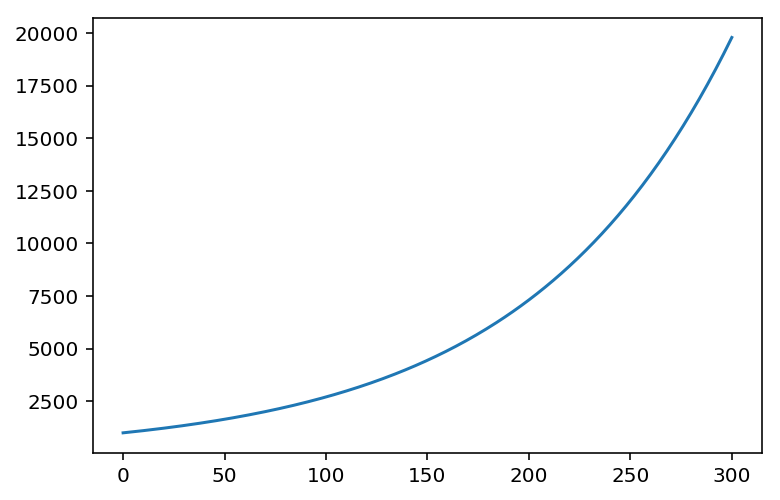
\includegraphics[width=8cm]{gs}
\end{center}

para encontrar este resultado, ocupamos que:

$$\sum_{i=0}^{n-1}a^i=\frac{1-n^{n}}{1-a}$$.


Algunos valores de la inversion:
\begin{center}
\begin{tabular}{|c|r|}
\hline
Mes & valor\\
\hline
0 & 1000\\
1 & 1010\\
2 & 1021.1\\
3 & 1030.301\\
\hline
\end{tabular}
\end{center}




\begin{center}
\huge
\textbf{NIÑOS NO HAGAN ESTO EN CASA.
pepe deja de ver mi pantalla!!!!!
y lupita }
\end{center}



sabemos que $\lim_{x\to\infty}\frac{1}{x}=0$.

calcular los valores propios de $$A=
\begin{pmatrix}
1 & 2\\
\pi & 4
\end{pmatrix}
.$$

\subsection{segundo orden}

\end{document}
